\documentclass{article}
\usepackage[english]{babel}

\usepackage[a4paper,top=2cm,bottom=2cm,left=3cm,right=3cm,marginparwidth=1.75cm]{geometry}
\usepackage{amsmath}
\usepackage{unicode-math}
\usepackage{graphicx}
\usepackage[colorlinks=true, allcolors=blue]{hyperref}
\usepackage{listings}
\usepackage{minted}
\usepackage{booktabs}
\usepackage{physics}
\usepackage{amssymb}%braket schreibweise
\setlength{\parindent}{0pt}

\title{Physics of Complex Systems: Exercise 9}
\author{Leopold Schaller and Daniel Lender}

\begin{document}
\maketitle

\section*{Task 9.1: Shannon entropy for binomial distribution}
\subsection*{(a)}
The Shannon entropy
\begin{align}
H(X) = -\sum_{i=1}^{n} P(x_i) \log_2 P(x_i)
\end{align}
is defined for a discrete variable $X$ and a probability distribution $P(x)$.
We use the following python function in a jupyter notebook to calculate the entropy:
\begin{minted}{python}
import numpy as np
from scipy.stats import binom, norm

def shannon_entropy_binomial(n, p=0.5):
    k = np.arange(0, n + 1)
    probabilities = binom.pmf(k, n, p)
    return -np.sum(probabilities * np.log2(probabilities))
\end{minted}

    We obtain the following entropies:
    \begin{align}
H (n=1) &= 1 \text{ bit} \\
H (2) &= 1.5 \text{ bit} \\
H (4) &= 2.0306 \text{ bit}  \\
H (8) &= 2.5442 \text{ bit}
    \end{align}
\subsection*{(b)}
For $p=\frac{1}{2}$ we obtain the following probability distribution:
$$P_n(k) = \binom{n}{k} \left(\frac{1}{2}\right)^n = \frac{n!}{k!(n-k)!} 2^{-n}$$
With the natural logarithm, we obtain a form where we can use the Stirling approximation:
$$\ln P_n(k) = \ln(n!) - \ln(k!) - \ln((n-k)!) - n \ln 2$$
Using the Stirling formula  $\ln(N!) \approx N \ln N - N $, we approximate this equation to
\begin{align}
    \ln P_n(k) & \approx \left[n\ln n - n \right] - \left[k\ln k - k\right] - \left[(n-k)\ln(n-k) - (n-k) \right] - n \ln 2 \\
               & \approx n\ln n - k\ln k - (n-k)\ln(n-k) - n\ln 2
\end{align}
For the Taylor expansion around the maximum $k_{max} = n/2$ for $f(x) =  \ln P_n(x)$, we shift $\ln P_n(x)$ by $k' = k - n/2$ and calculate some derivatives:
\begin{align}
f(x) &= - (x-\frac{n}{2})\ln (x-\frac{n}{2}) - (\frac{n}{2}-x)\ln(\frac{n}{2}-x) + C(n) \\
f'(x) &= \ln (x-\frac{n}{2}) - \ln (x+\frac{n}{2}) \\
f''(x) &= - \frac{1}{\frac{n}{2}-x} - \frac{1}{x+\frac{n}{2}} \\
f(0) &= \ln (\frac{n}{2}) (\frac{n}{2}-\frac{n}{2}) + C(n) = C(n) \\
f'(0) &= 0 \\
f''(0) &= - \frac{2}{n} - \frac{2}{n} = - \frac{4}{n}
\end{align}
With this values, we have all coefficients to perform the Taylor expansion until second order:
\begin{align}
    f(x) \approx C(n)  + 0 \cdot x - \frac{4}{n} \cdot  \frac{x^2}{2} = C(n) - \frac{2 x^2}{n}
\end{align}
The exponential of this results in our new approximation for the binomial distribution:
\begin{align}
    P_n(x) \approx C \exp^{-\frac{2 x^2}{n}}
\end{align}
We now have to normalize this continous distribution to obtain the correct factor $C$:
\begin{align}
    \int_{-\infty}^{\infty} P_n(x) \, dx &= 1 \implies C \int_{-\infty}^{\infty} e^{-\frac{2x^2}{n}} \, dx = C \sqrt{\frac{\pi n}{2}} = 1 \\
    C &= \sqrt{\frac{2}{\pi n}} \\
    P_n(x) &= \sqrt{\frac{2}{\pi n}} \exp^{-\frac{2 x^2}{n}}
\end{align}
The approximation and the exact distribution are plotted in Fig. \ref{figBinomial} for $n=50$.

\subsection{(c)}
The continous entropy with the natural logarithm is:
\begin{align}
    H &= -\int_{-\infty}^{\infty} p(x) \ln p(x) \, dx = -\int_{-\infty}^{\infty}  \sqrt{\frac{2}{\pi n}} \exp^{-\frac{2 x^2}{n}} \left( 0.5 \ln \frac{2}{\pi n} - \frac{2 x^2}{n} \right) dx \\
      &= - 0.5 \ln \frac{2}{\pi n} + \sqrt{\frac{2}{\pi n}} \frac{2}{n}  \left[ \int_{-\infty}^{\infty} \exp^{-\frac{2 x^2}{n}} x^2 dx \right] \\
      &= - 0.5 \ln \frac{2}{\pi n} + \sqrt{\frac{2}{\pi n}} \frac{2}{n} \left[ \sqrt{\frac{\pi n}{2}} \frac{n}{4} \right]\\
      &= - 0.5 \ln \frac{2}{\pi n} + \frac{1}{2} \\
      &=  0.5 \left( \ln n + \ln \frac{\pi}{2} + 1 \right)
\end{align}
If we want to convert this result into bit units, we have to multiply it with $\frac{1}{\ln 2}$ and obtain:
\begin{align}
    H_{bit} &=  0.5 \left( \frac{\ln n}{\ln 2} + \frac{\ln \frac{\pi}{2}}{\ln 2} + \frac{\ln e}{\ln 2} \right)
            &=  0.5 \left( \log_2 n + \log_2 \frac{\pi}{2} + \log_2 e \right)
            &=  0.5 \log_2 n + C
\end{align}
The result is compared with the exact Shannon entropy in \ref{figBinomial}. We observe good agreement.

\begin{figure}[]
    \centering
    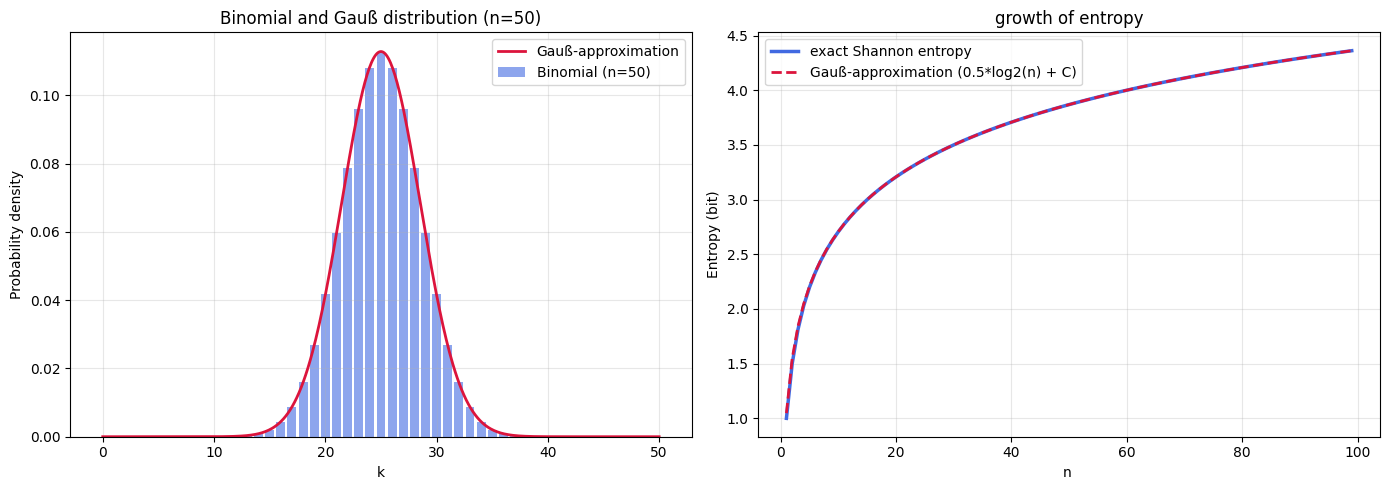
\includegraphics[width=1\linewidth]{Binomial.png}
    \caption{}
    \label{figBinomial}
\end{figure}

\end{document}

# pdflatex -shell-escape Uebung9/exercise9_Schaller_Lender.tex
